% =========================================================
% PHAN 11 -- CAU 10: MODEL IMPROVEMENT
% =========================================================

\section{Cải thiện mô hình (Model Improvement)}
\label{sec:model-improvement}

\subsection{Mục tiêu và thiết kế so sánh}

Kết quả hồi quy đơn biến ở Phần~\ref{sec:library-comparison}
cho thấy hai cách ước lượng tham số gần như tương đương,
nhưng mô hình chỉ giải thích được một phần nhỏ biến thiên
RTT đến máy chủ đích. Để cải thiện khả năng dự đoán, nhóm
triển khai ba hướng: mở rộng số đặc trưng, khảo sát các
thuật toán hồi quy tuyến tính và phi tuyến, và thử nghiệm
Gradient Descent kết hợp Momentum.

Phần này tổ chức ba thí nghiệm độc lập về mục đích:
\begin{enumerate}
    \item \textbf{Đánh giá trên tập kiểm tra cuối cùng:}
    so sánh chín mô hình trên cùng các quan sát kiểm tra.
    \item \textbf{So sánh theo quy mô dữ liệu huấn luyện:}
    huấn luyện chín mô hình ở sáu kích thước mẫu khác nhau,
    sử dụng một tập validation cố định và trực quan hóa kết quả
    bằng biểu đồ cột (bar chart).
    \item \textbf{Phân tích quá trình hội tụ và học theo bước:}
    ghi lại Training MSE và Validation MSE qua các vòng cập nhật
    hoặc boosting stage của năm mô hình có quy trình lặp phù hợp.
\end{enumerate}

Hai thí nghiệm sau chỉ sử dụng dữ liệu huấn luyện và validation;
nhóm giữ riêng tập kiểm tra cuối cùng để tránh sử dụng thông tin
kiểm tra trong quá trình khảo sát và lựa chọn mô hình.

\subsection{Chuẩn bị dữ liệu và bổ sung đặc trưng}

Nhóm lựa chọn bốn đặc trưng mạng làm đầu vào cho các mô hình
đa biến, như trình bày trong Bảng~\ref{tab:improvement-features}.

\begin{table}[H]
    \centering
    \caption{Các đặc trưng đầu vào của mô hình hồi quy đa biến}
    \label{tab:improvement-features}
    \small
    \begin{tabular}{p{0.48\textwidth}p{0.42\textwidth}}
        \toprule
        \textbf{Đặc trưng} & \textbf{Ý nghĩa} \\
        \midrule
        \texttt{gateway\_rtt\_avg\_ms} & RTT trung bình đến Gateway \\
        \texttt{tcp\_connect\_median\_ms} & Thời gian kết nối TCP trung vị \\
        \texttt{dns\_resolve\_ms} & Thời gian phân giải DNS \\
        \texttt{dns\_recursive\_ms} & Thời gian phân giải DNS đệ quy \\
        \bottomrule
    \end{tabular}
\end{table}

Nhóm sử dụng \texttt{rtt\_avg\_ms} làm biến mục tiêu.
Các mô hình đơn biến chỉ sử dụng đặc trưng
\texttt{gateway\_rtt\_avg\_ms}; các mô hình đa biến
sử dụng cả bốn đặc trưng trên.

Sau khi loại bỏ những quan sát thiếu dữ liệu ở các cột cần dùng,
tập dữ liệu có $54\,589$ mẫu. Nhóm thực hiện phép chia ngẫu nhiên
với \texttt{random\_state=42}: $43\,671$ mẫu huấn luyện ($80\%$)
và $10\,918$ mẫu kiểm tra ($20\%$). Nhóm huấn luyện lại cả hai
mô hình đơn biến trong thiết lập này; vì vậy tất cả chín mô hình
được đánh giá trên \textbf{cùng tập kiểm tra $10\,918$ mẫu}.

Với bốn đặc trưng $x_1,\ldots,x_4$, mô hình tuyến tính đa biến
ước lượng đầu ra theo phương trình:
\[
    \hat{y} = \theta_0 + \theta_1x_1 + \theta_2x_2
    + \theta_3x_3 + \theta_4x_4.
\]

\subsection{Các mô hình và cấu hình huấn luyện}

Nhóm so sánh chín mô hình, gồm hai mô hình đơn biến và bảy
mô hình đa biến. Bảng~\ref{tab:improvement-configurations}
trình bày cấu hình thực nghiệm được sử dụng.

\begin{table}[H]
    \centering
    \caption{Cấu hình chín mô hình trong thí nghiệm so sánh}
    \label{tab:improvement-configurations}
    \small
    \begin{tabular}{p{0.49\textwidth}p{0.42\textwidth}}
        \toprule
        \textbf{Mô hình} & \textbf{Cấu hình} \\
        \midrule
        NumPy GD (Univariate Baseline)
        & $\gamma=0.01$, $1000$ vòng lặp \\
        Scikit-learn LR (Univariate)
        & Ordinary Least Squares, có hệ số chặn \\
        Scikit-learn LR (Multivariate)
        & Ordinary Least Squares, có hệ số chặn \\
        Lasso Regression (L1)
        & \texttt{alpha=0.1} \\
        Ridge Regression (L2)
        & \texttt{alpha=1.0} \\
        Decision Tree Regressor
        & \texttt{max\_depth=8}, \texttt{min\_samples\_split=10} \\
        XGBoost Regressor
        & $100$ cây, learning rate $0.08$, \texttt{max\_depth=6} \\
        AdaBoost Regressor
        & $50$ bộ ước lượng, learning rate $0.1$ \\
        NumPy GD with Momentum (Multivariate)
        & $\gamma=0.01$, $\beta=0.9$, $1000$ vòng lặp \\
        \bottomrule
    \end{tabular}
\end{table}

Nhóm dùng Scikit-learn Linear Regression làm mốc tham chiếu
bình phương tối thiểu cho cả hai thiết lập đơn biến và đa biến.
Lasso và Ridge kiểm soát hệ số hồi quy bằng regularization
$L_1$ và $L_2$. Decision Tree, XGBoost và AdaBoost khai thác
các quan hệ phi tuyến giữa đặc trưng mạng và RTT đầu ra.

\subsection{Gradient Descent kết hợp Momentum}

Với mô hình NumPy GD with Momentum, nhóm chuẩn hóa từng
đặc trưng bằng thống kê của tập huấn luyện:
\[
    z_j^{(i)} =
    \frac{x_j^{(i)}-\mu_{j,\mathrm{train}}}
         {s_{j,\mathrm{train}}+10^{-8}},\qquad j=1,\ldots,4.
\]
Trong đó $\mu_{j,\mathrm{train}}$ và $s_{j,\mathrm{train}}$
lần lượt là trung bình và độ lệch chuẩn mẫu của đặc trưng
thứ $j$. Nhóm áp dụng chính các thống kê này cho tập validation
hoặc tập kiểm tra, không tính lại từ dữ liệu đánh giá.

Gọi $Z$ là ma trận thiết kế gồm cột hệ số chặn và bốn đặc trưng
đã chuẩn hóa. Hàm chi phí và gradient có dạng:
\[
    J(\boldsymbol{\theta})
    =\frac{1}{2n}\left\|Z\boldsymbol{\theta}-\mathbf{y}\right\|_2^2,
\]
\[
    \mathbf{g}^{(t)}
    =\frac{1}{n}Z^\top\left(Z\boldsymbol{\theta}^{(t)}-\mathbf{y}\right).
\]
Nhóm cập nhật vận tốc và tham số theo quy tắc Momentum:
\[
    \mathbf{v}^{(t+1)}
    =\beta\mathbf{v}^{(t)}+\gamma\mathbf{g}^{(t)},
\]
\[
    \boldsymbol{\theta}^{(t+1)}
    =\boldsymbol{\theta}^{(t)}-\mathbf{v}^{(t+1)}.
\]

Thí nghiệm sử dụng $\gamma=0.01$, $\beta=0.9$ và $1000$
vòng lặp. Chuẩn hóa hạn chế chênh lệch thang đo giữa các
đặc trưng; Momentum tích lũy thông tin từ các gradient trước
để điều chỉnh bước cập nhật.

\subsection{Kết quả trên tập kiểm tra cuối cùng}

Nhóm đánh giá chín mô hình bằng Mean Squared Error (MSE)
và hệ số xác định $R^2$ trên cùng tập kiểm tra $10\,918$ mẫu.
Bảng~\ref{tab:improvement-results} sắp xếp các mô hình theo
Test MSE tăng dần.

\begin{table}[H]
    \centering
    \caption{Kết quả chín mô hình trên cùng tập kiểm tra cuối cùng}
    \label{tab:improvement-results}
    \small
    \begin{tabular}{p{0.57\textwidth}rr}
        \toprule
        \textbf{Mô hình} & \textbf{Test MSE ($\mathrm{ms}^2$)}
        & $\boldsymbol{R^2}$ \\
        \midrule
        Decision Tree Regressor & \textbf{16.3844} & \textbf{0.5431} \\
        XGBoost Regressor & 20.5236 & 0.4276 \\
        AdaBoost Regressor & 21.5279 & 0.3996 \\
        Lasso Regression (L1) & 31.8263 & 0.1124 \\
        Ridge Regression (L2) & 31.8609 & 0.1114 \\
        Scikit-learn LR (Multivariate) & 31.8610 & 0.1114 \\
        NumPy GD with Momentum & 31.8610 & 0.1114 \\
        Scikit-learn LR (Univariate) & 34.9150 & 0.0263 \\
        NumPy GD (Univariate Baseline) & 34.9155 & 0.0262 \\
        \bottomrule
    \end{tabular}
\end{table}

\paragraph{So sánh các mô hình tuyến tính.}

Hai phương pháp đơn biến đạt Test MSE gần như bằng nhau:
$34.9155$ với NumPy GD và $34.9150$ với Scikit-learn LR.
Khi mở rộng lên bốn đặc trưng, Scikit-learn LR giảm Test MSE
xuống $31.8610$ và tăng $R^2$ lên khoảng $0.1114$.
Lasso, Ridge và NumPy GD with Momentum đạt kết quả rất gần
mô hình tuyến tính đa biến. Điều này xác nhận cách tối ưu
Gradient Descent kết hợp Momentum thu được nghiệm dự đoán
gần tương đương nghiệm tuyến tính của thư viện.

\paragraph{So sánh các mô hình phi tuyến.}

Decision Tree Regressor đạt Test MSE thấp nhất, $16.3844$,
và $R^2$ cao nhất, $0.5431$. So với Scikit-learn LR đa biến,
Decision Tree giảm MSE khoảng $48.58\%$.
XGBoost và AdaBoost lần lượt đạt Test MSE $20.5236$ và
$21.5279$. Cả ba mô hình phi tuyến đều có MSE thấp hơn nhóm
tuyến tính trong phép chia dữ liệu này. Kết quả cho thấy
các quan hệ phi tuyến giữa đặc trưng mạng và RTT đóng vai trò
quan trọng đối với khả năng dự đoán.

% =========================================================
% PHAN 11A -- TRAINING-SIZE PERFORMANCE COMPARISON
% =========================================================

\subsection{So sánh hiệu năng theo quy mô dữ liệu huấn luyện}
\label{subsec:training-size-comparison}

\paragraph{Thiết kế thực nghiệm.}

Để kiểm tra ảnh hưởng của số lượng mẫu đến chất lượng dự đoán,
nhóm tiếp tục chia $43\,671$ quan sát huấn luyện thành
\textit{training pool} gồm $34\,936$ mẫu ($80\%$) và
\textit{validation set} cố định gồm $8\,735$ mẫu ($20\%$),
với \texttt{random\_state=42}.
Nhóm giữ nguyên tập kiểm tra cuối cùng $10\,918$ mẫu,
không sử dụng tập này trong phép so sánh theo quy mô.

Nhóm tạo sáu tập con lồng nhau từ training pool bằng một
hoán vị ngẫu nhiên cố định. Mỗi tập lớn hơn bao gồm toàn bộ
các quan sát của tập nhỏ hơn. Nhóm huấn luyện lại từ đầu cả
chín mô hình trên từng tập con, sau đó tính Training MSE
trên tập con tương ứng và Validation MSE trên cùng
$8\,735$ quan sát validation.

\begin{table}[H]
    \centering
    \caption{Sáu quy mô dữ liệu huấn luyện dùng trong thí nghiệm}
    \label{tab:learning-curve-sizes}
    \small
    \begin{tabular}{rr}
        \toprule
        \textbf{Tỷ lệ training pool} & \textbf{Số mẫu huấn luyện} \\
        \midrule
        $10\%$  & 3\,493 \\
        $20\%$  & 6\,987 \\
        $40\%$  & 13\,974 \\
        $60\%$  & 20\,961 \\
        $80\%$  & 27\,948 \\
        $100\%$ & 34\,936 \\
        \bottomrule
    \end{tabular}
\end{table}

Thí nghiệm này \textbf{thay đổi số lượng mẫu huấn luyện},
không thay đổi số bước tối ưu khi tính từng điểm kết quả.
Vì vậy, các bảng và biểu đồ cột sau đây thể hiện mức độ nhạy
của hiệu năng với quy mô dữ liệu; chúng không phải đường
hội tụ theo số vòng lặp của thuật toán.

\paragraph{Biểu đồ so sánh theo quy mô dữ liệu.}

Hình~\ref{fig:training-size-bar-chart} gồm sáu biểu đồ cột ngang,
mỗi biểu đồ tương ứng một tỷ lệ training pool và so sánh
chín mô hình theo Training MSE và Validation MSE.
Nhóm sắp xếp mô hình theo Validation MSE tăng dần ở từng mức
để người đọc xác định trực tiếp phương pháp dự đoán tốt nhất.

\begin{figure}[H]
    \centering
    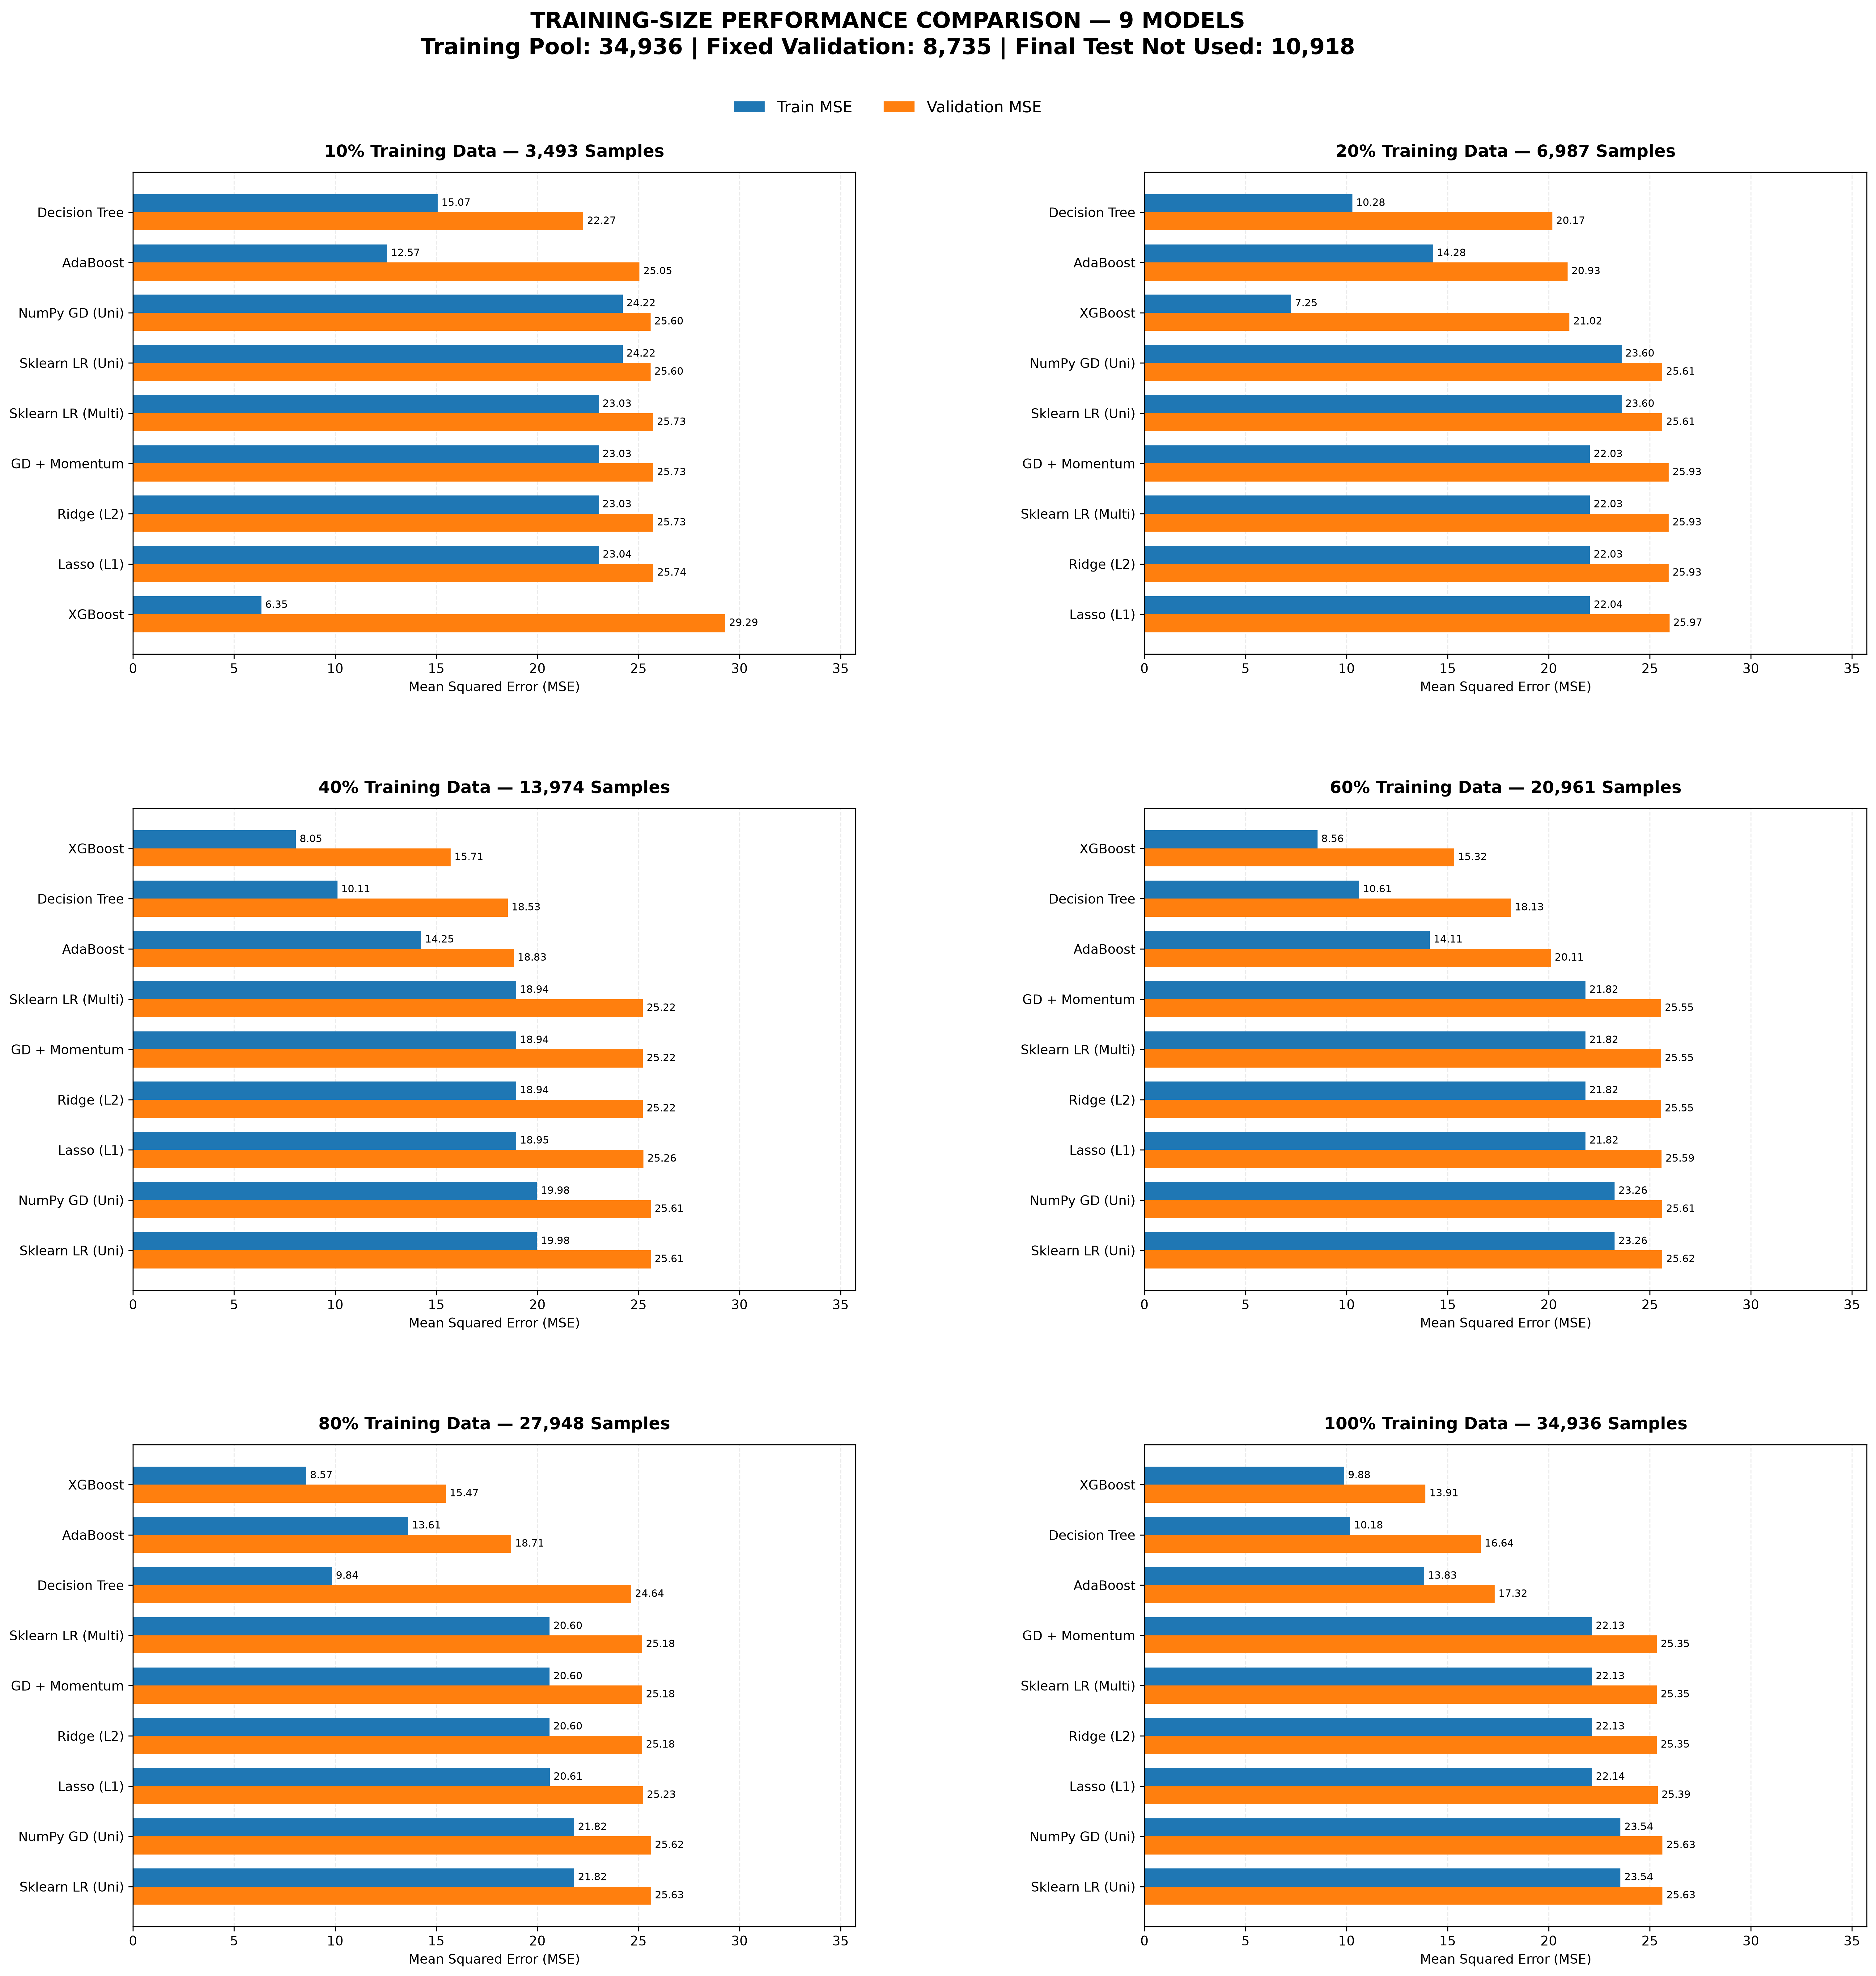
\includegraphics[width=0.98\textwidth]
    {Task10_Training_Size_Performance_Bar_Chart_9_Models.png}
    \caption{So sánh Training MSE và Validation MSE của chín mô hình
    ở sáu quy mô dữ liệu huấn luyện (Training-Size Performance Comparison).
    Cả sáu biểu đồ sử dụng cùng tập validation cố định.}
    \label{fig:training-size-bar-chart}
\end{figure}

\paragraph{Kết quả định lượng.}

Bảng~\ref{tab:lc-10} đến Bảng~\ref{tab:lc-100} trình bày
các kết quả số tương ứng với Hình~\ref{fig:training-size-bar-chart}.
Mỗi bảng xếp chín mô hình theo Validation MSE tăng dần;
Training MSE phản ánh mức độ khớp trên tập huấn luyện,
trong khi Validation MSE đánh giá khả năng dự đoán trên
những quan sát không dùng để cập nhật mô hình.

% =========================================================
% TRAINING-SIZE COMPARISON -- 10% TRAINING POOL
% =========================================================

\begin{table}[H]
    \centering
    \caption{So sánh hiệu năng với $10\%$ training pool ($3\,493$ mẫu)}
    \label{tab:lc-10}
    \small
    \begin{tabular}{r p{0.47\textwidth} rr}
        \toprule
        \textbf{Hạng} & \textbf{Mô hình} & \textbf{Train MSE}
        & \textbf{Val. MSE} \\
        \midrule
        1 & Decision Tree & 15.0668 & \textbf{22.2689} \\
        2 & AdaBoost & 12.5676 & 25.0474 \\
        3 & NumPy GD (đơn biến) & 24.2198 & 25.5997 \\
        4 & Scikit-learn LR (đơn biến) & 24.2198 & 25.6004 \\
        5 & Scikit-learn LR (đa biến) & 23.0342 & 25.7271 \\
        6 & NumPy GD + Momentum & 23.0342 & 25.7271 \\
        7 & Ridge (L2) & 23.0342 & 25.7272 \\
        8 & Lasso (L1) & 23.0424 & 25.7430 \\
        9 & XGBoost & 6.2210 & 27.5821 \\
        \bottomrule
    \end{tabular}
\end{table}

% =========================================================
% TRAINING-SIZE COMPARISON -- 20% TRAINING POOL
% =========================================================

\begin{table}[H]
    \centering
    \caption{So sánh hiệu năng với $20\%$ training pool ($6\,987$ mẫu)}
    \label{tab:lc-20}
    \small
    \begin{tabular}{r p{0.47\textwidth} rr}
        \toprule
        \textbf{Hạng} & \textbf{Mô hình} & \textbf{Train MSE}
        & \textbf{Val. MSE} \\
        \midrule
        1 & XGBoost & 7.1266 & \textbf{18.3136} \\
        2 & Decision Tree & 10.2838 & 20.1750 \\
        3 & AdaBoost & 14.2760 & 20.9297 \\
        4 & NumPy GD (đơn biến) & 23.6004 & 25.6134 \\
        5 & Scikit-learn LR (đơn biến) & 23.6004 & 25.6136 \\
        6 & NumPy GD + Momentum & 22.0332 & 25.9343 \\
        7 & Scikit-learn LR (đa biến) & 22.0332 & 25.9343 \\
        8 & Ridge (L2) & 22.0332 & 25.9343 \\
        9 & Lasso (L1) & 22.0384 & 25.9703 \\
        \bottomrule
    \end{tabular}
\end{table}

% =========================================================
% TRAINING-SIZE COMPARISON -- 40% TRAINING POOL
% =========================================================

\begin{table}[H]
    \centering
    \caption{So sánh hiệu năng với $40\%$ training pool ($13\,974$ mẫu)}
    \label{tab:lc-40}
    \small
    \begin{tabular}{r p{0.47\textwidth} rr}
        \toprule
        \textbf{Hạng} & \textbf{Mô hình} & \textbf{Train MSE}
        & \textbf{Val. MSE} \\
        \midrule
        1 & XGBoost & 8.1635 & \textbf{16.0626} \\
        2 & Decision Tree & 10.1101 & 18.5322 \\
        3 & AdaBoost & 14.2518 & 18.8307 \\
        4 & NumPy GD + Momentum & 18.9446 & 25.2195 \\
        5 & Scikit-learn LR (đa biến) & 18.9446 & 25.2195 \\
        6 & Ridge (L2) & 18.9446 & 25.2195 \\
        7 & Lasso (L1) & 18.9510 & 25.2569 \\
        8 & NumPy GD (đơn biến) & 19.9789 & 25.6128 \\
        9 & Scikit-learn LR (đơn biến) & 19.9789 & 25.6130 \\
        \bottomrule
    \end{tabular}
\end{table}

% =========================================================
% TRAINING-SIZE COMPARISON -- 60% TRAINING POOL
% =========================================================

\begin{table}[H]
    \centering
    \caption{So sánh hiệu năng với $60\%$ training pool ($20\,961$ mẫu)}
    \label{tab:lc-60}
    \small
    \begin{tabular}{r p{0.47\textwidth} rr}
        \toprule
        \textbf{Hạng} & \textbf{Mô hình} & \textbf{Train MSE}
        & \textbf{Val. MSE} \\
        \midrule
        1 & XGBoost & 8.4477 & \textbf{14.7485} \\
        2 & Decision Tree & 10.6127 & 18.1291 \\
        3 & AdaBoost & 14.1111 & 20.1050 \\
        4 & Scikit-learn LR (đa biến) & 21.8173 & 25.5502 \\
        5 & NumPy GD + Momentum & 21.8173 & 25.5502 \\
        6 & Ridge (L2) & 21.8173 & 25.5502 \\
        7 & Lasso (L1) & 21.8241 & 25.5863 \\
        8 & NumPy GD (đơn biến) & 23.2571 & 25.6148 \\
        9 & Scikit-learn LR (đơn biến) & 23.2571 & 25.6152 \\
        \bottomrule
    \end{tabular}
\end{table}

% =========================================================
% TRAINING-SIZE COMPARISON -- 80% TRAINING POOL
% =========================================================

\begin{table}[H]
    \centering
    \caption{So sánh hiệu năng với $80\%$ training pool ($27\,948$ mẫu)}
    \label{tab:lc-80}
    \small
    \begin{tabular}{r p{0.47\textwidth} rr}
        \toprule
        \textbf{Hạng} & \textbf{Mô hình} & \textbf{Train MSE}
        & \textbf{Val. MSE} \\
        \midrule
        1 & XGBoost & 8.7181 & \textbf{14.5523} \\
        2 & AdaBoost & 13.6064 & 18.7114 \\
        3 & Decision Tree & 9.8443 & 24.6413 \\
        4 & Scikit-learn LR (đa biến) & 20.6033 & 25.1818 \\
        5 & NumPy GD + Momentum & 20.6033 & 25.1818 \\
        6 & Ridge (L2) & 20.6033 & 25.1818 \\
        7 & Lasso (L1) & 20.6105 & 25.2281 \\
        8 & NumPy GD (đơn biến) & 21.8172 & 25.6250 \\
        9 & Scikit-learn LR (đơn biến) & 21.8172 & 25.6255 \\
        \bottomrule
    \end{tabular}
\end{table}

% =========================================================
% TRAINING-SIZE COMPARISON -- 100% TRAINING POOL
% =========================================================

\begin{table}[H]
    \centering
    \caption{So sánh hiệu năng với $100\%$ training pool ($34\,936$ mẫu)}
    \label{tab:lc-100}
    \small
    \begin{tabular}{r p{0.47\textwidth} rr}
        \toprule
        \textbf{Hạng} & \textbf{Mô hình} & \textbf{Train MSE}
        & \textbf{Val. MSE} \\
        \midrule
        1 & XGBoost & 9.8632 & \textbf{14.4839} \\
        2 & Decision Tree & 10.1773 & 16.6417 \\
        3 & AdaBoost & 13.8318 & 17.3199 \\
        4 & Scikit-learn LR (đa biến) & 22.1330 & 25.3474 \\
        5 & NumPy GD + Momentum & 22.1330 & 25.3474 \\
        6 & Ridge (L2) & 22.1330 & 25.3474 \\
        7 & Lasso (L1) & 22.1395 & 25.3908 \\
        8 & NumPy GD (đơn biến) & 23.5436 & 25.6319 \\
        9 & Scikit-learn LR (đơn biến) & 23.5436 & 25.6323 \\
        \bottomrule
    \end{tabular}
\end{table}


\paragraph{Ảnh hưởng của quy mô mẫu đến chất lượng dự đoán.}

Tại $10\%$ training pool, Decision Tree đạt Validation MSE thấp
nhất ($22.2689$); XGBoost đạt Training MSE chỉ $6.2210$ nhưng
Validation MSE lên tới $27.5821$. Chênh lệch này phản ánh dấu
hiệu overfitting khi XGBoost học từ tập con nhỏ.

Từ mức $20\%$ training pool, XGBoost dẫn đầu về Validation MSE.
Sai số của mô hình giảm từ $18.3136$ ở $20\%$ xuống $16.0626$
ở $40\%$, $14.7485$ ở $60\%$, $14.5523$ ở $80\%$
và $14.4839$ ở $100\%$. Ở mức $100\%$, XGBoost đạt
Training MSE $9.8632$ và Validation MSE $14.4839$;
khoảng cách giữa hai chỉ số nhỏ hơn rõ rệt so với mức $10\%$.

Decision Tree đạt Validation MSE $16.6417$ ở $100\%$ training pool,
nhưng sai số không giảm đều khi số lượng mẫu tăng. Tại $80\%$,
Validation MSE tăng lên $24.6413$ rồi giảm ở $100\%$.
Biến động này cho thấy kết quả của cây quyết định phụ thuộc
vào thành phần dữ liệu huấn luyện, ngay cả khi các tập con
được tạo theo cấu trúc lồng nhau.

Nhóm mô hình tuyến tính đa biến có Validation MSE tương đối gần
nhau. Ở mức $100\%$, Scikit-learn LR đa biến, Ridge và
NumPy GD with Momentum cùng đạt xấp xỉ $25.3474$,
còn Lasso đạt $25.3908$. Hai mô hình đơn biến đạt
Validation MSE lần lượt $25.6319$ (NumPy GD) và $25.6323$
(Scikit-learn LR). Việc bổ sung đặc trưng làm giảm sai số
của nhóm tuyến tính nhưng chưa đạt được mức dự đoán của
các mô hình phi tuyến.

Tại $100\%$ training pool, thứ hạng validation lần lượt
bắt đầu bằng XGBoost ($14.4839$), Decision Tree ($16.6417$)
và AdaBoost ($17.3199$). Tuy nhiên, trên tập kiểm tra cuối
cùng, Decision Tree đứng đầu. Sự khác biệt giữa validation
và test nhấn mạnh rằng xếp hạng ở một phép chia dữ liệu
không bảo đảm giữ nguyên khi thay đổi tập đánh giá.

% =========================================================
% PHAN 11B -- CONVERGENCE / TRAINING-STAGE ANALYSIS
% =========================================================

\subsection{Phân tích hội tụ và tiến trình học của các mô hình}
\label{subsec:iterative-convergence}

\paragraph{Thiết lập và cách đọc biểu đồ.}

Để quan sát diễn biến sai số trong quá trình huấn luyện, nhóm
sử dụng toàn bộ training pool $34\,936$ mẫu và tập validation
cố định $8\,735$ mẫu. Nhóm ghi nhận Training MSE và Validation
MSE sau từng bước cập nhật đối với năm mô hình có quy trình
lặp thích hợp: NumPy GD đơn biến, NumPy GD with Momentum đa biến,
XGBoost, AdaBoost và Lasso.

Số vòng lặp mang ý nghĩa khác nhau giữa các thuật toán.
Với hai mô hình GD, một bước tương ứng một lần cập nhật gradient
trên toàn tập; với XGBoost và AdaBoost, một bước là một vòng
bổ sung bộ học yếu; với Lasso, nhóm theo dõi các lượt
coordinate descent. Vì vậy, nhóm trình bày mỗi mô hình trên
một hệ trục riêng, không dùng chung trục số vòng lặp để so sánh
trực tiếp tốc độ hội tụ giữa các thuật toán.

Đối với Lasso, \texttt{Scikit-learn} không cung cấp sẵn lịch sử
MSE theo từng vòng tối ưu. Nhóm dựng lại tiến trình bằng cách
huấn luyện liên tiếp với \texttt{warm\_start=True} và
\texttt{max\_iter=1}; đường cong này là một thí nghiệm
bổ sung, \textbf{không phải lịch sử được lưu từ lần huấn luyện
Lasso ở bảng kết quả test}. Nhóm đồng thời ghi lại duality gap
trên thang logarit để theo dõi tiến độ tối ưu hàm mục tiêu
có regularization.

\begin{figure}[H]
    \centering
    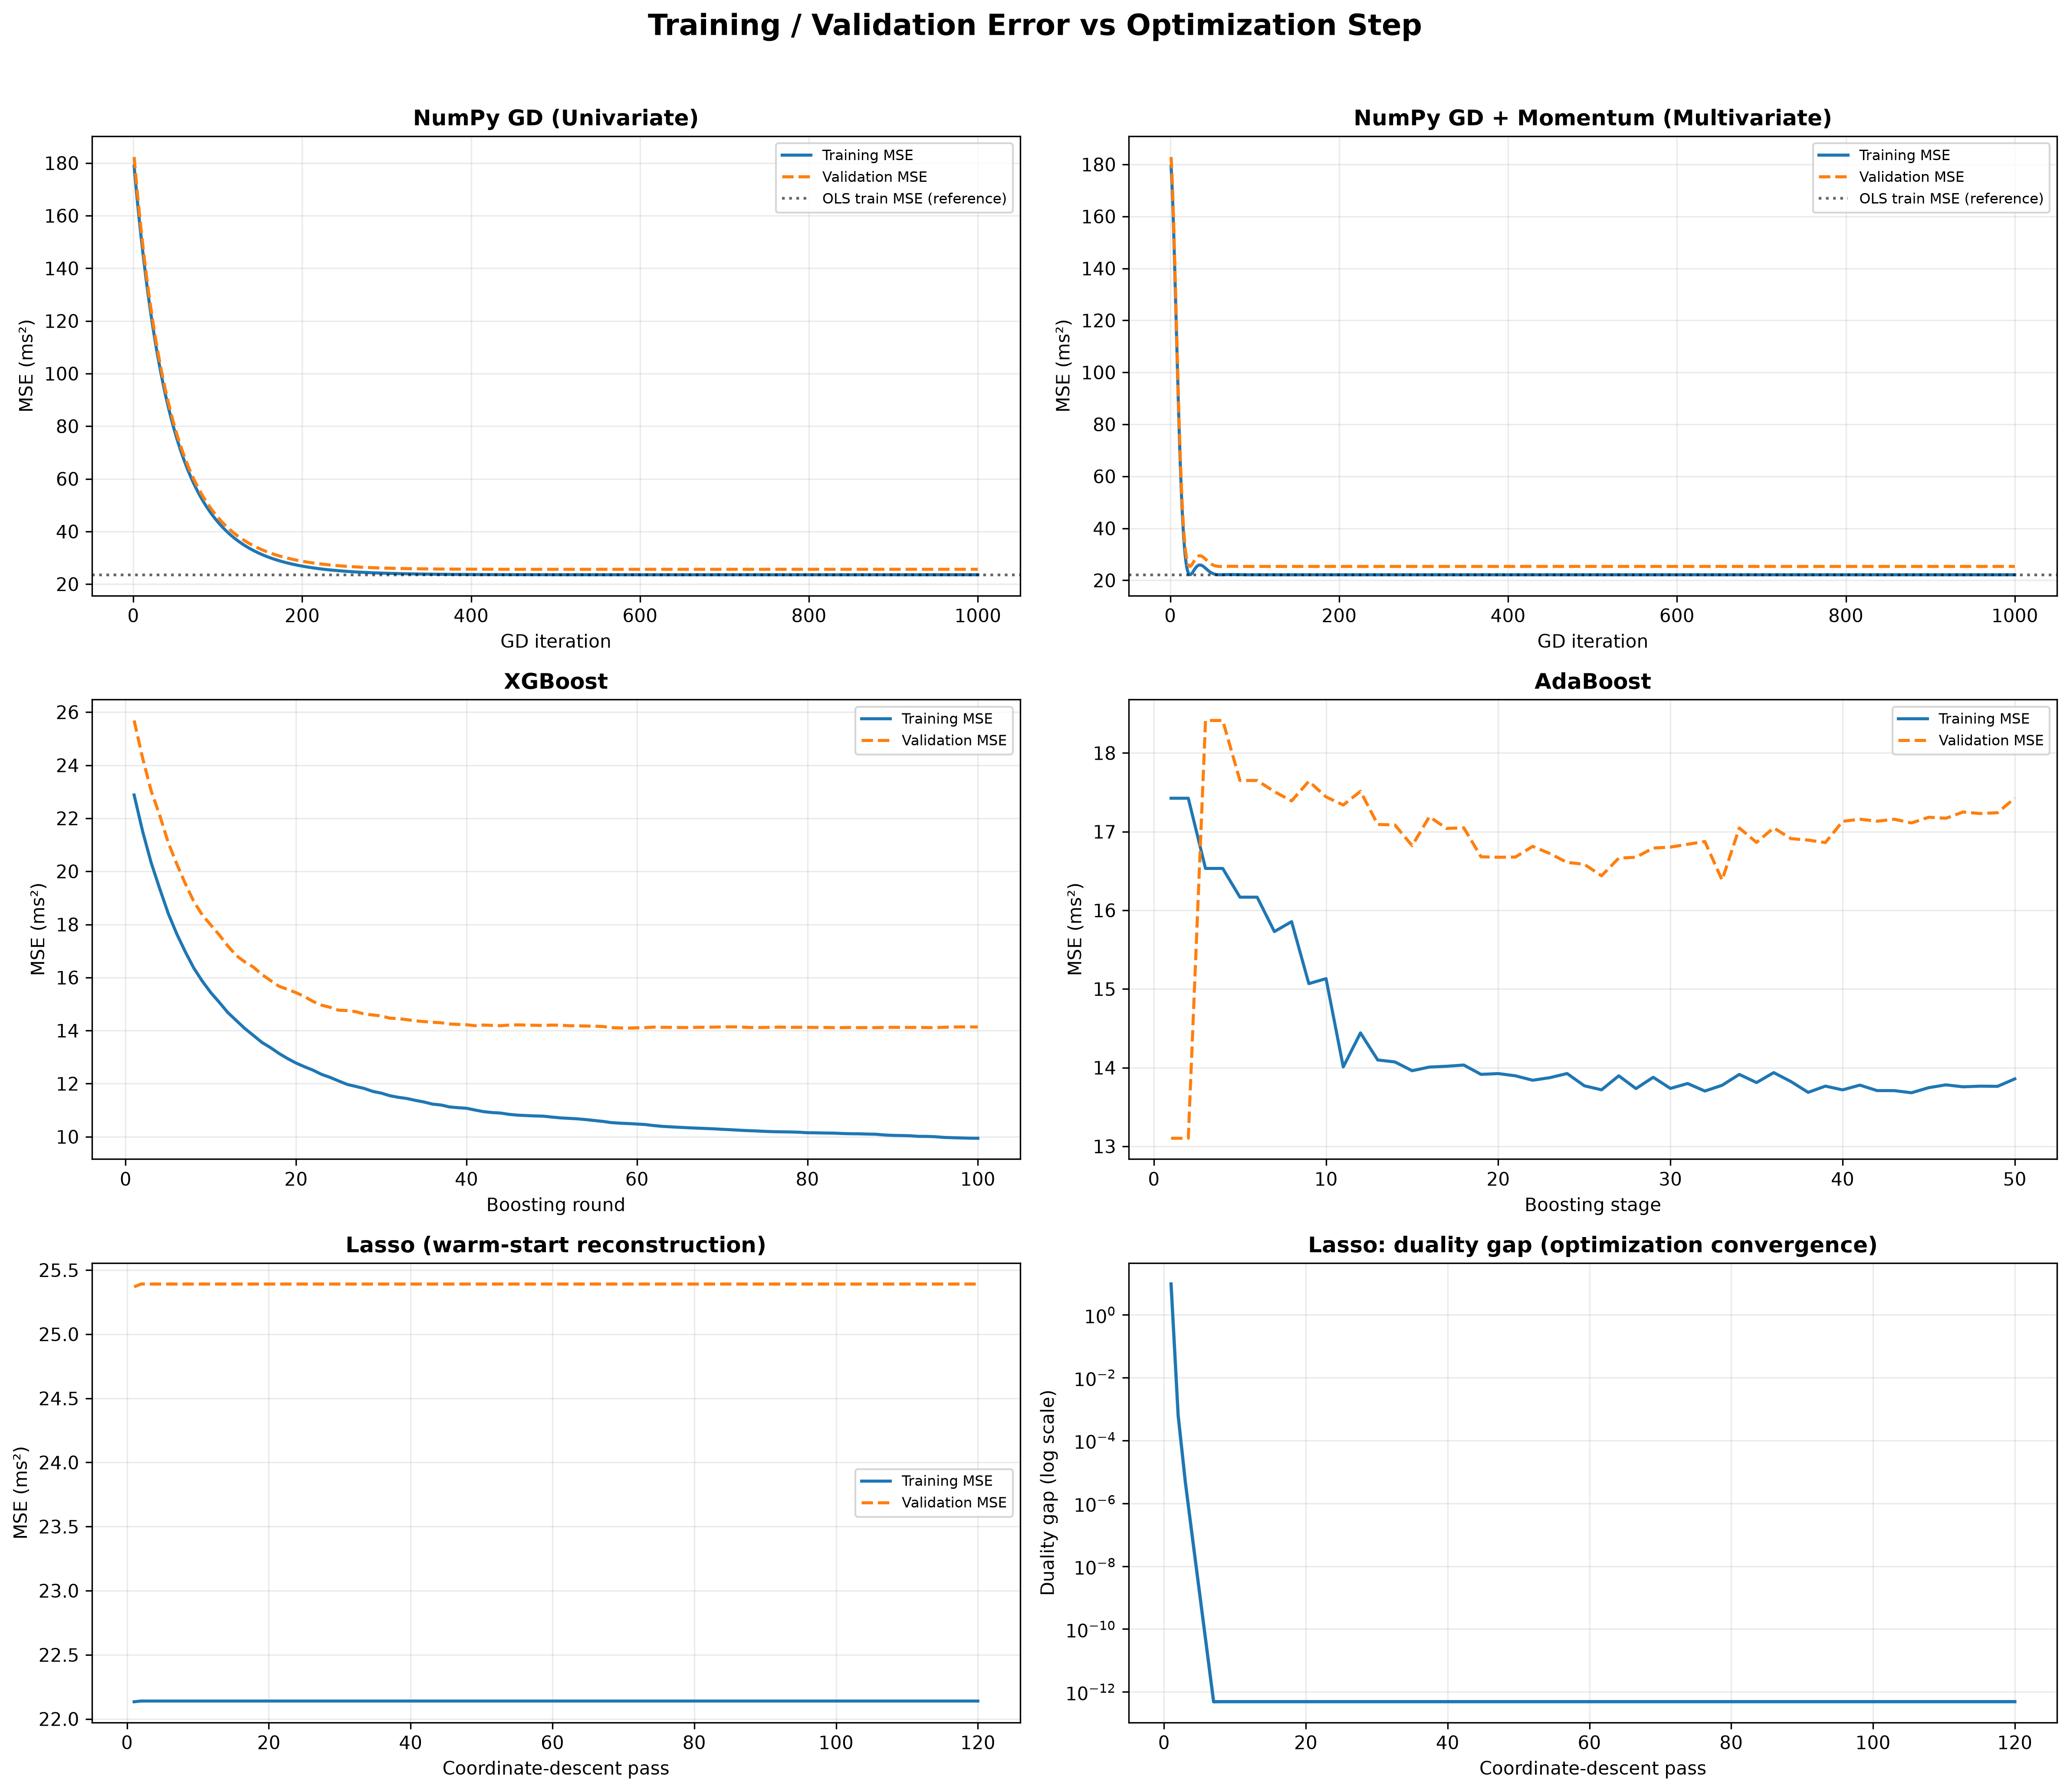
\includegraphics[width=0.98\textwidth]
    {Task10_Convergence_5_Iterative_Models.png}
    \caption{Diễn biến Training MSE và Validation MSE theo bước huấn luyện
    của năm mô hình lặp. Ô cuối biểu diễn duality gap của Lasso
    theo các lượt coordinate descent. Các đường OLS trong hai ô GD
    làm mốc sai số huấn luyện của nghiệm bình phương tối thiểu.}
    \label{fig:improvement-convergence}
\end{figure}

\paragraph{Kết quả định lượng.}

Bảng~\ref{tab:improvement-convergence} tổng hợp số bước
và MSE ở bước cuối cùng của từng phép huấn luyện phục vụ
biểu đồ hội tụ.

\begin{table}[H]
    \centering
    \caption{Sai số ở bước cuối của các thí nghiệm theo dõi hội tụ}
    \label{tab:improvement-convergence}
    \small
    \begin{tabular}{p{0.43\textwidth}rrr}
        \toprule
        \textbf{Mô hình} & \textbf{Số bước} & \textbf{Train MSE}
        & \textbf{Val. MSE} \\
        \midrule
        NumPy GD (đơn biến) & 1000 & 23.5436 & 25.6319 \\
        NumPy GD + Momentum (đa biến) & 1000 & 22.1330 & 25.3474 \\
        XGBoost & 100 & 9.6875 & 14.4129 \\
        AdaBoost & 50 & 13.8567 & 17.4270 \\
        Lasso (warm-start) & 120 & 22.1395 & 25.3908 \\
        \bottomrule
    \end{tabular}
\end{table}

\paragraph{Nhận xét quá trình tối ưu.}

Ở mô hình NumPy GD đơn biến, Training MSE và Validation MSE
giảm mạnh trong những vòng lặp đầu và tiến đến vùng ổn định.
Hai đường nằm gần nhau, trong khi Training MSE tiệm cận mốc
OLS của mô hình đơn biến. Với Gradient Descent kết hợp Momentum,
sai số giảm nhanh hơn ở giai đoạn đầu, sau đó ổn định gần
mốc OLS đa biến. Hai biểu đồ xác nhận quá trình cập nhật
tham số tiến gần nghiệm tuyến tính tương ứng.

Với XGBoost, Training MSE tiếp tục giảm khi số vòng boosting
tăng, còn Validation MSE giảm nhanh ở giai đoạn đầu rồi
đi vào vùng ổn định. Ở vòng thứ $100$, mô hình đạt Training MSE
$9.6875$ và Validation MSE $14.4129$. Khoảng cách còn lại
phản ánh độ chênh giữa khả năng khớp dữ liệu huấn luyện
và khả năng dự đoán trên validation.

Với AdaBoost, Training MSE nhìn chung giảm theo các boosting
stage nhưng Validation MSE dao động. Ở stage thứ $50$,
Training MSE đạt $13.8567$ và Validation MSE đạt $17.4270$.
Điều này cho thấy việc thêm bộ học yếu không nhất thiết
làm Validation MSE giảm đều ở mọi stage.

Với Lasso, Training MSE và Validation MSE gần như ổn định
từ những lượt coordinate descent đầu. Duality gap giảm nhanh
về gần không, xác nhận bộ giải tiến gần nghiệm của
bài toán tối ưu có regularization. Giá trị hàm mục tiêu
regularized giảm từ khoảng $11.145761$ ở lượt đầu xuống
$11.143954$ ở lượt cuối.

\textit{Phân biệt hai kiểu biểu đồ.}
Biểu đồ cột ở Hình~\ref{fig:training-size-bar-chart} thay đổi
\textbf{số lượng mẫu huấn luyện} và so sánh các mô hình tại
sáu mức dữ liệu. Hình~\ref{fig:improvement-convergence}
quan sát \textbf{sai số theo từng bước huấn luyện} trên một
quy mô dữ liệu cố định. Với XGBoost và AdaBoost, các đường
này theo dõi hiệu năng dự đoán theo boosting stage; chúng
không tự thân chứng minh hội tụ đến nghiệm tối ưu toàn cục.

Các kết quả XGBoost và AdaBoost ở Bảng~\ref{tab:improvement-convergence}
có sai khác nhỏ so với hàng $100\%$ trong Bảng~\ref{tab:lc-100}
do biểu đồ hội tụ sử dụng một lượt huấn luyện riêng, trong khi
thí nghiệm quy mô mẫu sắp xếp lại các hàng của training pool.
Nhóm giữ nguyên giá trị ghi nhận từ từng thí nghiệm và
không sử dụng hai bảng này như những lần đo trùng nhau.

\subsection{Kết luận}

Thử nghiệm trên cùng tập kiểm tra cho thấy Decision Tree
Regressor đạt kết quả tốt nhất trong chín mô hình,
với MSE $16.3844$ và $R^2=0.5431$.
Nhóm mô hình tuyến tính đa biến cải thiện so với hai mô hình
đơn biến, nhưng các thuật toán phi tuyến đạt sai số thấp hơn.

Khi tăng quy mô training pool, XGBoost cải thiện Validation MSE
rõ rệt và đạt giá trị thấp nhất $14.4839$ ở mức $100\%$.
Tuy nhiên, kết quả cuối cùng trên test vẫn ưu tiên Decision Tree,
cho thấy cần phân biệt khả năng dự đoán trên validation
với đánh giá độc lập trên test.

Các đường theo dõi tối ưu cung cấp thông tin bổ sung:
Gradient Descent và Gradient Descent with Momentum tiến gần
nghiệm OLS, XGBoost và AdaBoost thể hiện mức thay đổi sai số
qua các boosting stage, còn duality gap xác nhận tiến độ
hội tụ của Lasso.

Kết quả được ghi nhận với một phép chia dữ liệu và bộ siêu
tham số cố định. Các thí nghiệm tiếp theo cần kiểm tra độ
ổn định trên nhiều phép chia, lựa chọn siêu tham số qua
validation và đánh giá theo thứ tự thời gian để phù hợp hơn
với bản chất chuỗi thời gian của dữ liệu mạng.